\apendice{Especificación de diseño}

\section{Introducción}
En esta sección se detallan los aspectos más importantes de la aplicación: los datos utilizados, los procedimientos de la aplicación, la arquitectura de la aplicación y el diseño de las interfaces.

\section{Diseño de datos} \label{datos}
Los datos utilizados para el desarrollo de la aplicación no quedan más allá del almacenamiento de los usuarios en una base de datos y el procesamiento del vídeo.

Dado que la aplicación desarrollada cuenta con alta, modificación y baja de usuarios, así como la obligación de estar dado de alta para utilizar la aplicación, esta debe estar conectada con una base de datos para almacenar los datos de los usuarios. La base de datos cuenta con una única tabla donde se almacena la información de los usuarios agregados, siguiendo la siguiente estructura de columnas:

\begin{itemize}
	\item \textbf{id:} es el identificador único del usuario. En la base de datos es una clave primaria.
	\item \textbf{usuario:} es el nombre de usuario que se utilizará para iniciar sesión. Debe ser único para cada usuario, por lo que en la base de datos es un UNIQUE.
	\item \textbf{contraseña:} es la contraseña utilizada para iniciar sesión junto al usuario correspondiente. Dado que la contraseña debe ser secreta, en la base de datos se guarda encriptada.
	\item \textbf{nombre\_completo:} es el nombre completo del usuario. Su utilidad es dar la bienvenida al usuario que inicie sesión en la aplicación.
\end{itemize}

Para realizar la predicción, se debe procesar el vídeo subido al servidor. Los datos obtenidos para predecir son los mismos que se utilizaron en la fase de investigación. Estos son: las amplitudes normalizadas, la velocidad media, la mano y el sexo. Una vez obtenidas las características, se utilizan en el modelo entrenado previamente para realizar la predicción.

\section{Diseño procedimental}
En ese apartado se detalla el procedimiento que se sigue a la hora de utilizar la aplicación web. Para ello, se ha dibujado el diagrama de secuencia de la figura~\ref{fig:diagrama_secuencia}, con los pasos que hay que seguir para realizar una predicción.

Hay varias aclaraciones que son necesarias indicar sobre este diagrama:

\begin{itemize}
	\item El actor que realiza las operaciones de inicio de sesión y predicción es el usuario que está en la aplicación. Se diferencia de la clase usuario (:Usuario), que es la clase que implementa el objeto del usuario y las operaciones relacionadas con él.
	\item El error en el acceso puede manifestarse de dos maneras: usuario inválido o contraseña inválida.
	\item El error en la subida puede manifestarse de dos maneras: formato de vídeo no válido o se deben rellenar los campos.
	\item El usuario conectado se corresponde con el permiso que tiene el usuario que acaba de introducir sus datos de acceso, que será diferente si es administrador, y le da acceso a las pantallas de la aplicación que no se pueden acceder sin iniciar sesión previamente.
	\item El paso ``7: obtener\_datos'' está formado por pasos internos en los que se calculan las características que requieren operaciones de cálculo. Contiene la extracción de: las amplitudes, los tiempos, las velocidades y la normalización.
\end{itemize}

\begin{figure}[ht]
	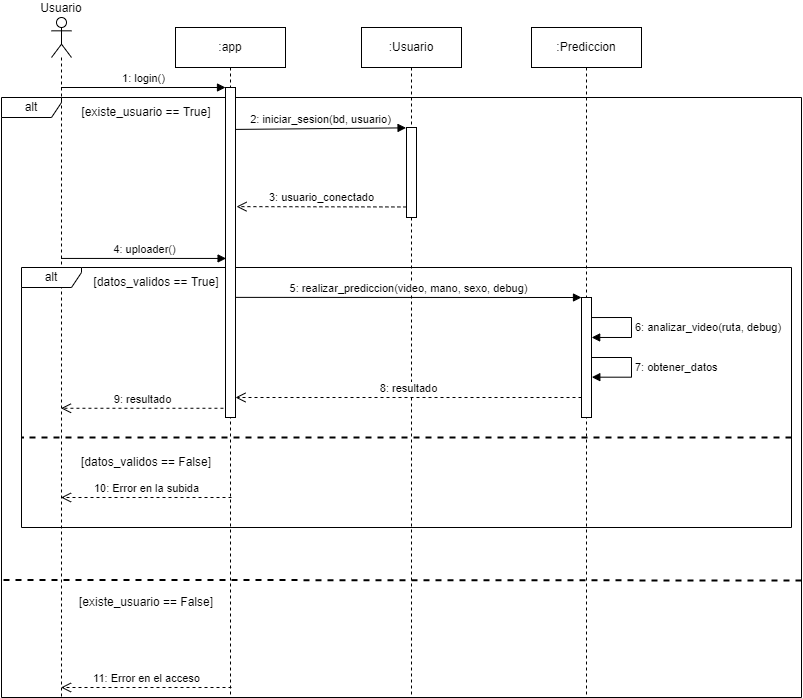
\includegraphics[width=1\textwidth]{diagrama_secuencia}
	\caption{Diagrama de secuencia de la predicción.}
	\label{fig:diagrama_secuencia}
\end{figure}

\section{Diseño arquitectónico}
En esta sección se detalla cómo es la arquitectura de la aplicación. La aplicación se divide en 6 principales componentes, cuya relación entre ellos viene representada en el diagrama de la figura \ref{fig:diagrama_componentes}:

\begin{itemize}
	\item \textbf{Cliente:} es el único componente que no está en el lado del servidor. El cliente se corresponde al navegador que realiza la petición al servidor solicitando recursos.
	\item \textbf{app:} es el servidor de la aplicación. Representa el núcleo debido a que todos los componentes, a excepción de la base de datos, están conectados a él. Cuando un cliente solicite un recurso (\textit{e. g.} una predicción), este componente comunicará los datos de la solicitud al componente \textit{Prediccion} para obtener un resultado y poder enviar la respuesta al cliente.
	\item \textbf{Prediccion:} es el componente dedicado a realizar el procesado del vídeo y la predicción de los datos obtenidos. Para ello, obtiene el vídeo, la mano y el sexo que le llega al servidor por parte del cliente, del vídeo obtiene el resto de características para entrenar el modelo configurado y finalmente realiza la predicción. Esa predicción vuelve al núcleo del servidor para enviar la respuesta al cliente.
	\item \textbf{Gestion\_usuarios:} es el componente dedicado a la gestión de los usuarios. Todas las operaciones de la gestión de usuarios (alta, modificación y baja), se realizan mediante consultas SQL. Por esta razón, existe conexión con la base de datos.
	\item \textbf{Usuario:} es el componente que instancia el usuario que se conecta a la aplicación, permitiéndole utilizar todas las funcionalidades al alcance de sus privilegios. También está conectado a la base de datos porque necesita comprobar que el usuario que está iniciando sesión está dado de alta en la aplicación y que su contraseña es la correcta.
	\item \textbf{Base de datos:} en ella se almacena toda la información ya descrita en el apartado \ref{datos} de este documento.
\end{itemize}

\begin{figure}[ht]
	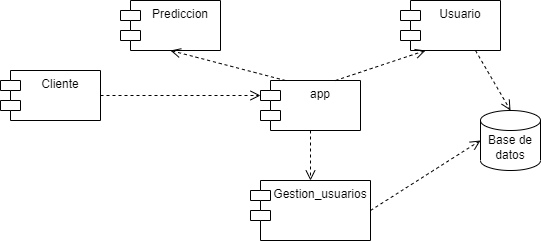
\includegraphics[width=1\textwidth]{diagrama_componentes}
	\caption{Diagrama de componentes de la aplicación web.}
	\label{fig:diagrama_componentes}
\end{figure} 

\section{Diseño de interfaces}
En este apartado, se muestran los diseños realizados de la aplicación web con la función de mostrar las funcionalidades que tendría la aplicación web, además de mostrar una interfaz con aspecto amigable.

\subsection{Vista de usuario}
Las pantallas del usuario son idénticas a las del administrador con la diferencia de que los usuarios no tendrán las opciones de ``Gestionar usuarios'' y ``Modificar modelo'', en su lugar tendrán la opción ``Modificar usuario''. Además, tendrán ventanas restringidas a las que únicamente el usuario administrador podrá acceder. Las ventanas disponibles para los usuarios sin privilegios son las correspondientes a las figuras \ref{fig:inicio_de_sesion}, \ref{fig:inicio}, \ref{fig:resultado} y \ref{fig:modificar_usuario}.

\subsection{Vista de administrador}
Se muestra el diseño de las interfaces para un usuario con privilegios.
\begin{figure}[h]
	\frame{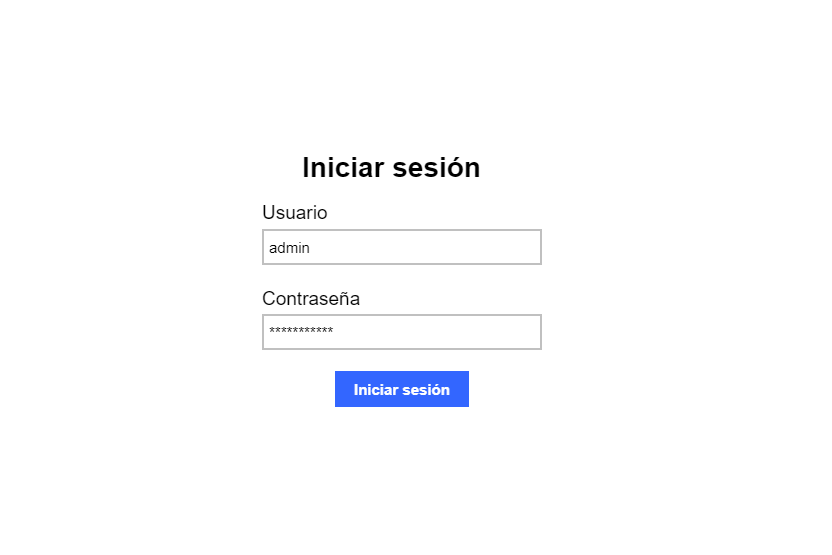
\includegraphics[width=1\textwidth]{inicio_de_sesion_admin}}
	\caption{Pantalla de inicio de sesión de un usuario administrador.}
	\label{fig:inicio_de_sesion}
\end{figure}

\begin{figure}[h]
	\frame{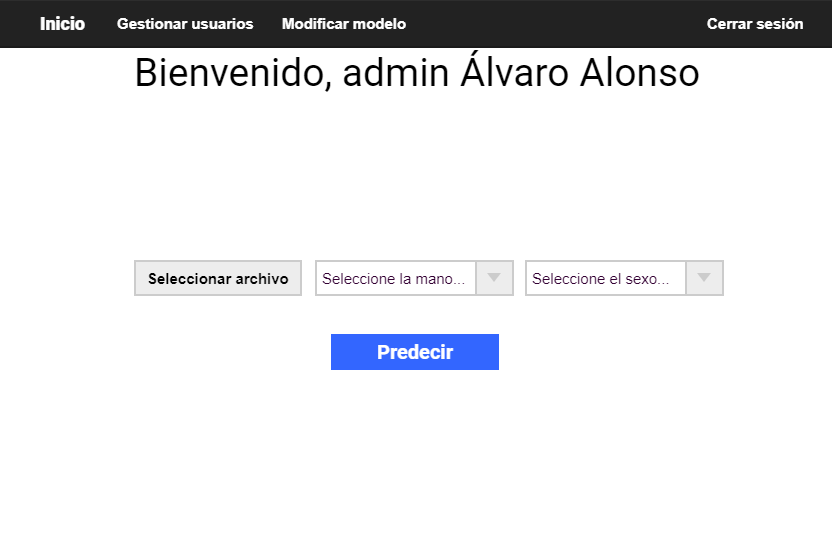
\includegraphics[width=1\textwidth]{inicio_admin}}
	\caption{Pantalla inicial de un usuario administrador.}
	\label{fig:inicio}
\end{figure}

\begin{figure}[h]
	\frame{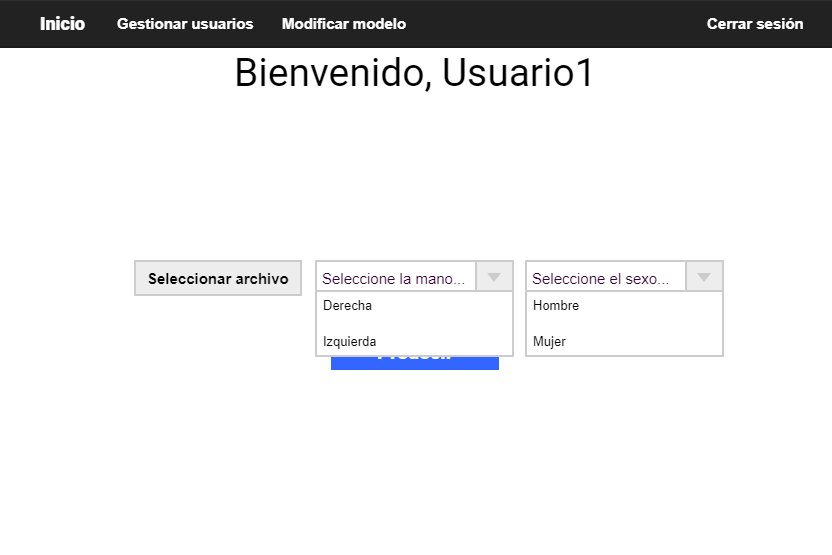
\includegraphics[width=1\textwidth]{inicio_admin_1}}
	\caption{Pantalla inicial de un usuario administrador con las listas desplegadas.}
	\label{fig:inicio_1}
\end{figure}

\begin{figure}[h]
	\frame{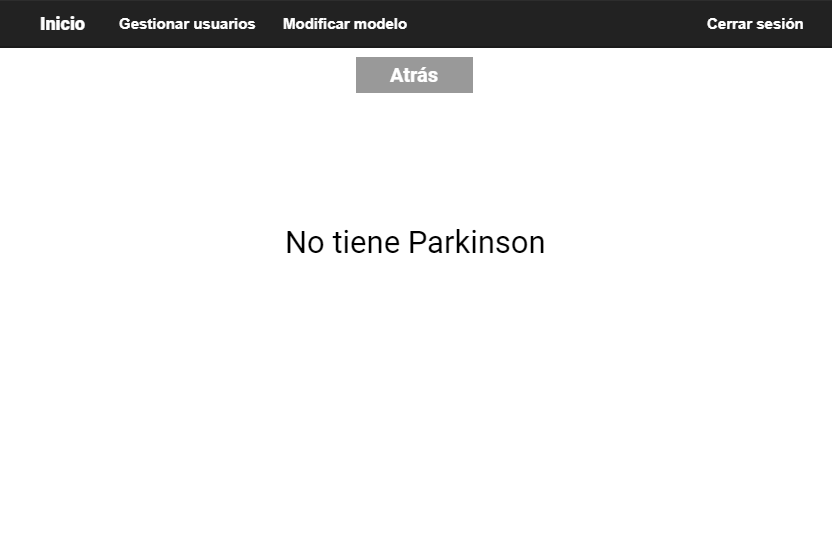
\includegraphics[width=1\textwidth]{resultado_admin}}
	\caption{Pantalla con el resultado de la predicción de un usuario administrador.}
	\label{fig:resultado}
\end{figure}

\begin{figure}[h]
	\frame{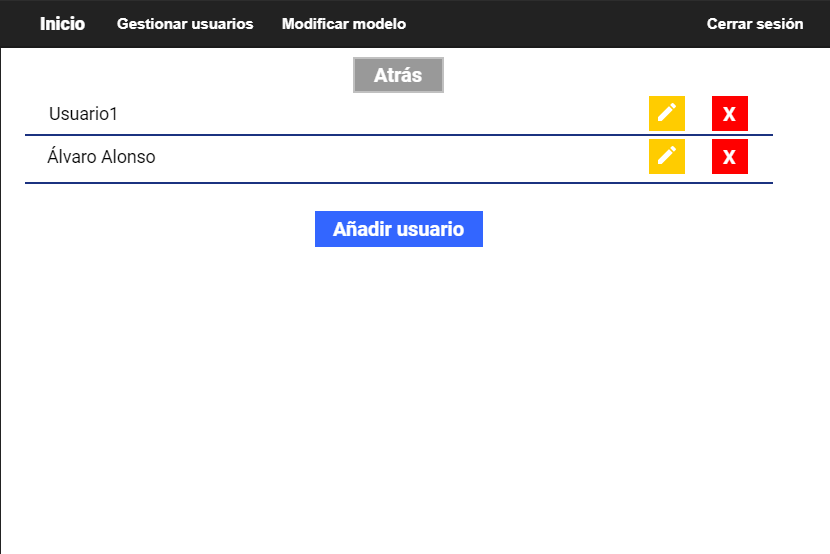
\includegraphics[width=1\textwidth]{gestionar_usuarios}}
	\caption{Pantalla con el listado de los usuarios dados de alta en la aplicación.}
	\label{fig:gestionar_usuarios}
\end{figure}

\begin{figure}[h]
	\frame{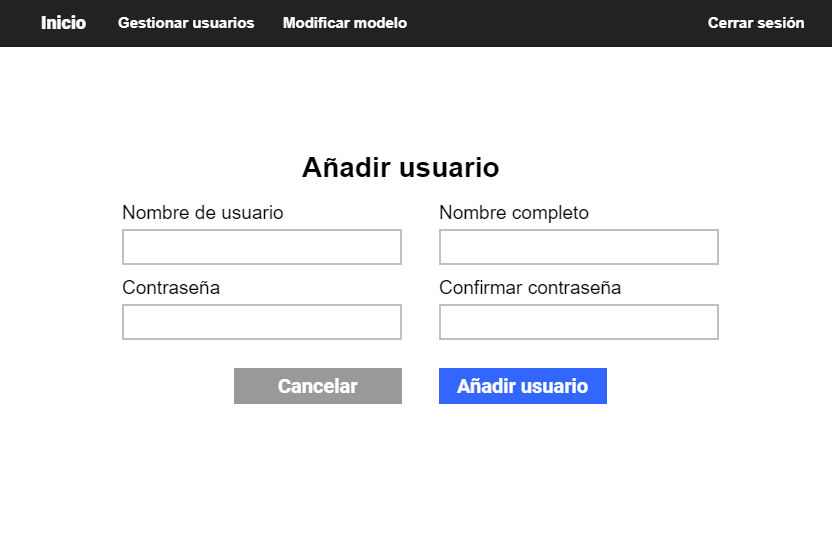
\includegraphics[width=1\textwidth]{agregar_usuario}}
	\caption{Pantalla con el formulario para dar de alta a un usuario.}
	\label{fig:agregar_usuario}
\end{figure}

\begin{figure}[h]
	\frame{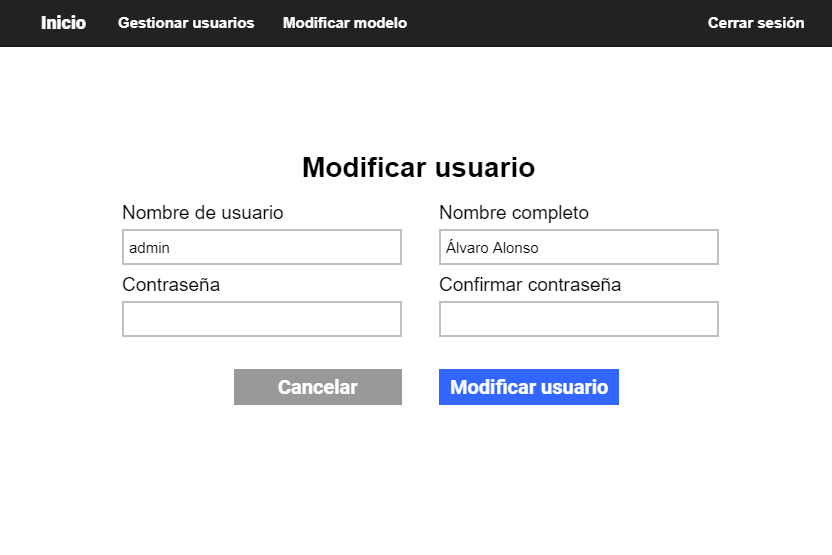
\includegraphics[width=1\textwidth]{modificar_usuario}}
	\caption{Pantalla con el formulario para modificar un usuario existente.}
	\label{fig:modificar_usuario}
\end{figure}

\begin{figure}[h]
	\frame{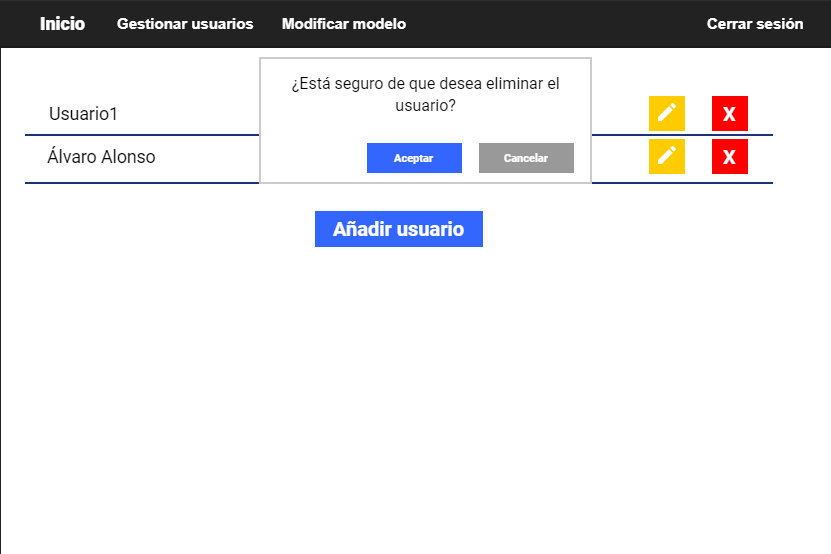
\includegraphics[width=1\textwidth]{eliminar_usuario}}
	\caption{Pantalla con la confirmación para borrar el usuario.}
	\label{fig:eliminar_usuario}
\end{figure}

\begin{figure}[h]
	\frame{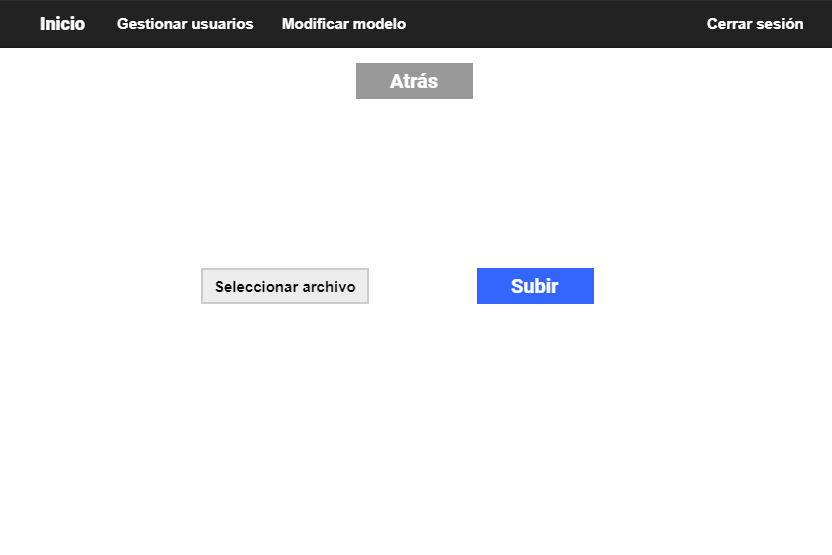
\includegraphics[width=1\textwidth]{modificar_modelo}}
	\caption{Pantalla con la subida del modelo al servidor.}
	\label{fig:modificar_modelo}
\end{figure}
